\documentclass{article}
\usepackage[utf8]{inputenc}
\usepackage{tikz}
\usetikzlibrary{shapes.geometric, arrows}
\renewcommand\familydefault{\sfdefault}

\tikzstyle{startstop} = [rectangle, rounded corners, text width=3cm, minimum width=3cm, minimum height=1cm,text centered, draw=black, fill=red!50]

\tikzstyle{io} = [trapezium, trapezium left angle=70, trapezium right angle=110, text width=3cm, minimum width=3cm, minimum height=1cm, text centered, draw=black, fill=blue!50]

\tikzstyle{process} = [rectangle, text width=3cm, minimum width=3cm, minimum height=1cm, text centered, draw=black, fill=orange!70]

\tikzstyle{decision} = [diamond, text width=3cm, minimum width=3cm, minimum height=1cm, text centered, draw=black, fill=green!50]

\tikzstyle{arrow} = [thick,->,>=stealth]

\begin{document}
\pagenumbering{gobble}
\section*{\centering{Server Message Handling}}

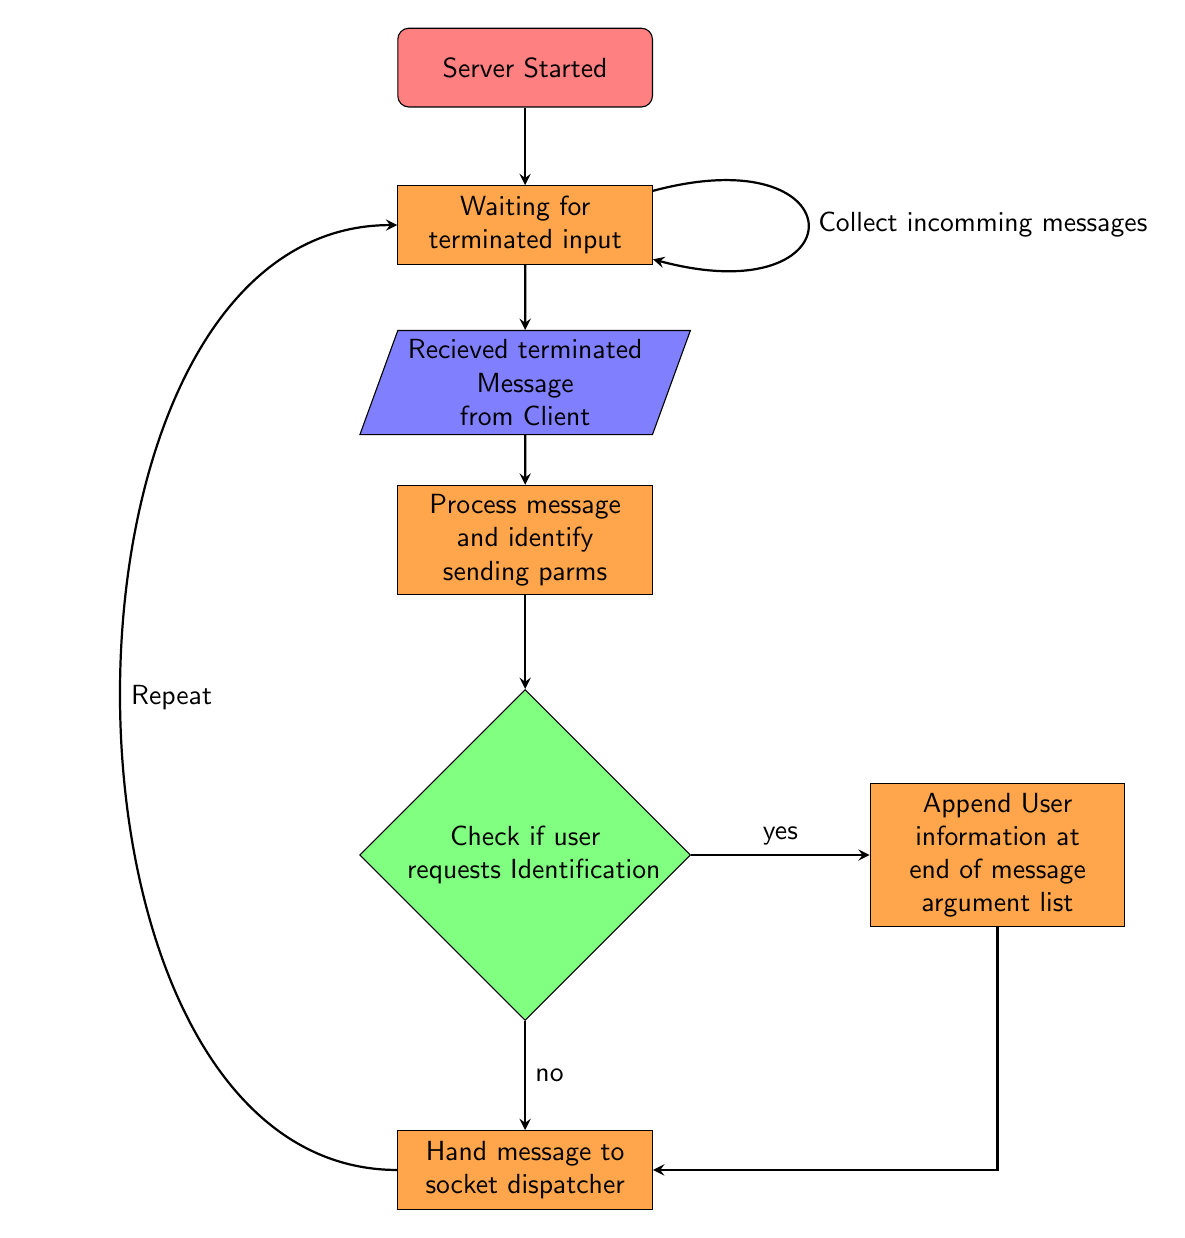
\begin{tikzpicture}[node distance=2cm]

\node (start) [startstop] {Server Started};
\node (ioLoop) [process, below of=start] {Waiting for terminated input};
\node (messageArrived) [io, below of=ioLoop] {Recieved \mbox{terminated} Message from Client};
\node (processMessage) [process, below of=messageArrived] {Process message and identify sending parms};
\node (identifyUser) [decision, yshift=-2cm, below of=processMessage] {Check if user \mbox{requests Identification}};
\node (sendOf) [process, yshift=-2cm, below of=identifyUser] {Hand message to socket dispatcher};
\node (userInfo) [process, xshift=4cm, right of=identifyUser] {Append User information at end of message argument list};

\draw [arrow] (start) -- (ioLoop);
\draw [arrow, loop right] (ioLoop) to node [anchor=west] {Collect incomming messages} (ioLoop);
\draw [arrow] (ioLoop) -- (messageArrived);
\draw [arrow] (messageArrived) -- (processMessage);
\draw [arrow] (processMessage) -- (identifyUser);
\draw [arrow] (identifyUser) -- node [anchor=south] {yes} (userInfo);
\draw [arrow] (identifyUser) -- node [anchor=west] {no} (sendOf);
\draw [arrow] (userInfo) |- (sendOf);
\draw [arrow, out=180, in=180] (sendOf) to node [anchor=west] {Repeat} (ioLoop);

\end{tikzpicture}

\end{document}